\chapter{Evaluation}


% The S2Store is implemented as explained in Chapter \ref{chap:design}. Our expectations are explained in \emph{Hypothesis} and compared to the experimental outcome in \emph{Results}.
%
%
% \section{Design}
%
% The application architecture is pictured as below:

\section{Design}

The S2Store is based on the following architecture.
% TODO: Insert architecture image here
% TODO: basic blocks - how it hooks up to the rest of the architecture
% Languages used, layers, etc

To answer the research questions mentioned in \ref{sec:questions-to-be-answered}, we use Artificial Life model inspired from the paper \cite{lim2012successful}. Similar to ``AppEco'' mentioned in the paper, which is an artificial life model for mobile ecosystem,  it to add extra actor models to adapt it to the architecture of S2Store so it fits the requirements of smart space store.

\section{Objective and Setup}

Different online platforms uses different types of reputation models with varying success. These platforms also have varying requirements. The closest we can compare S2Store is to either Apple's App Store or Google's Play Store. The basic functioning of S2Store is similar to the mobile app store. However it also has additional features that differs from mobile platforms. \cite{lim2012successful} created ``AppEco'', which is an Artificial Life modeling to see the behavior of

\textbf{RQ1}: Can a reputation system separate the good, average and bad quality of applications?

\textbf{RQ2}: How do convergence behave under different reputation systems and which one is effective compared to another?

\textbf{RQ3}: Can convergence work for all three: services, context models and access groups?

\textbf{RQ4}: Does ``editor picked list'' improve convergence in terms of time and quality?

\textbf{RQ5}: Does ``versioning'' of services, context models and access groups improve convergence in terms of time and quality?

Evaluation

\section{Implementation}

\subsection{Technical Architecture}

\begin{figure}[!htb]
  \centering
  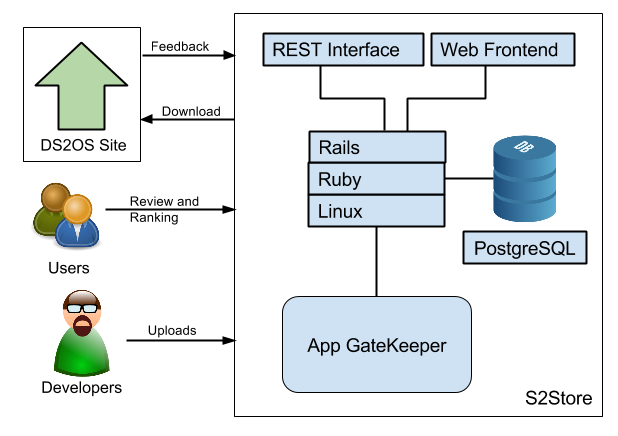
\includegraphics[width=14cm]{figures/technical_architecture.png}
  \caption{Technical Architecture}
  \label{fig:technical-architecture}
\end{figure}

S2Store is implemented in Ruby on Rails web framework\footnote{http://rubyonrails.org/}. It is programmed in Ruby\footnote{https://www.ruby-lang.org/en/} language and runs in a linux environment. It uses PostgreSQL\footnote{http://www.postgresql.org/} to store any data. It provides two types of interfaces:

\begin{enumerate}
  \item \textbf{REST Interface}: DS2OS Sites communicate via REST Inteface to download services, submit feedback for application status and feedbacks whenever there are any kind of crashes.
  \item \textbf{Web Interface}: Users and Developers use the web frontend via a browser to interact with the S2Store. It allows users to register, upload applications, search and rate applications in the S2Store.
\end{enumerate}

\subsection{Components Architecture}

\begin{figure}[!htb]
  \centering
  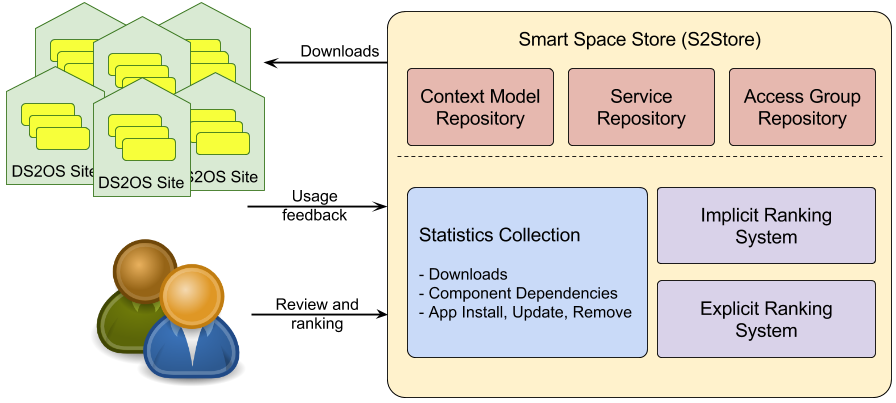
\includegraphics[width=15cm]{figures/components_architecture.png}
  \caption{Components Architecture}
  \label{fig:components-architecture}
\end{figure}

  * Figure
  * Explanation of each parts (Each part should contain)
    * What it is
    * What it does
    * Interaction with other system, entities, users

* Artificial Life (Alife) agent-based modeling
  * APPECO for S2Store
  * AppEco components
  * Devs
    * Explain
  * Entities
    * Explain
    * Interdependencies
    * Explicit vs Implicit Reputations
  * Users
  * Reputation System Update
  * App Store
  * AppEco Algorithm

* Expectaiton
  * Distribution Graph

* Experiments
  * Calibration
  * Setup

* Result and Analysis
  *

* Conslusion
